\section{\emph{Holonomic Robot}}
\label{sec:holonomicrobot}

\emph{Holonomic robot} merupakan jenis robot yang memiliki kemampuan untuk bergerak secara \emph{holonomic},
  yakni sebuah kondisi dimana jumlah \emph{degree of freedom} (DoF) yang dapat dikendalikan sama dengan total DoF yang dimiliki.
Salah satu bentuk dari \emph{holonomic robot} adalah robot dengan roda \emph{omni-directional}.
Robot jenis ini memiliki kemampuan manuver yang bagus dan efisien dengan mengorbankan kompleksitas pada desain pergerakan robot.
Menurut \citet{cit:oliveira2008},
  sebuah robot dengan tiga atau lebih roda \emph{omni-directional} mampu memiliki kemampuan pergerakan tangensial, normal, dan \emph{angular} secara hampir independen ke segala arah.

\emph{Robot holonomic} dengan roda \emph{omni-directional} pada umumnya memiliki tiga hingga empat buah roda.
Robot dengan tiga buah roda secara mekanik memiliki desain yang lebih sederhana,
  namun dengan adanya empat buah roda,
  robot dapat memiliki akselerasi yang lebih tinggi sembari mengurangi kemungkinan adanya \emph{wheel slippage}.

\begin{figure}[ht]
  \centering
  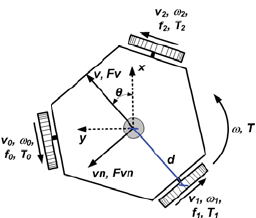
\includegraphics[height=0.3\textwidth,keepaspectratio]{gambar/diagram-robot-tiga-roda.png}
  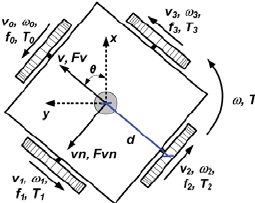
\includegraphics[height=0.3\textwidth,keepaspectratio]{gambar/diagram-robot-empat-roda.png}
  \caption{Diagram kinematik robot dengan tiga dan empat roda \emph{omni-directional} \citep{cit:oliveira2008}.}
  \label{fig:diagramkinematikrobot}
\end{figure}

Pada robot dengan roda \emph{omni-directional},
  model kinematik robot dapat dibentuk seperti pada gambar \ref{fig:diagramkinematikrobot}.
Dari gambar tersebut, dihasilkan persamaan \ref{eq:kinematikrobotroda3} untuk robot dengan tiga buah roda dan persamaan \ref{eq:kinematikrobotroda4} untuk robot dengan empat buah roda.
Pada persamaan tersebut,
  $v_{i}$ merupakan kecepatan setiap motor roda yang dimiliki robot,
  $v(t)$ dan $vn(t)$ merupakan kecepatan liniear robot,
  dan $w(t)$ merupakan kecepatan putar robot.

\begin{equation}
  \label{eq:kinematikrobotroda3}
  \begin{bmatrix}
  v_{0} \\ v_{1} \\ v_{2}
\end{bmatrix}
=
\begin{bmatrix}
  -sin(\pi / 3) & cos(\pi / 3) & d \\
  0 & -1 & d \\
  sin(\pi / 3) & cos(\pi / 3) & d
\end{bmatrix}
\begin{bmatrix}
  v(t) \\ vn(t) \\ \omega(t)
\end{bmatrix}

\end{equation}

\begin{equation}
  \label{eq:kinematikrobotroda4}
  \begin{bmatrix}
  v_{0} \\ v_{1} \\ v_{2} \\ v_{3}
\end{bmatrix}
=
\begin{bmatrix}
  0 & 1 & d \\
  -1 & 0 & d \\
  0 & -1 & d \\
  1 & 0 & d
\end{bmatrix}
\begin{bmatrix}
  v(t) \\ vn(t) \\ \omega(t)
\end{bmatrix}

\end{equation}
